\documentclass[12pt]{jarticle}
\usepackage{TUSIReport}
\usepackage{otf}
\usepackage[dvipdfmx]{graphicx}
\usepackage[dvipdfmx]{color}
\usepackage{amsmath}
\usepackage{amssymb}
\usepackage{color}
\usepackage{hhline}
\usepackage{fancybox,ascmac}
\usepackage{multirow}
\usepackage{url}
\usepackage{bm}
\usepackage{listings,jlisting}
\lstdefinestyle{log}{
    frame={tblr},
    basicstyle={\footnotesize},
    tabsize={4},
}
\lstdefinestyle{lstcpp}{
    language={c++},
    backgroundcolor={\color[gray]{.85}},
    basicstyle={\small},
    identifierstyle={\small},
    commentstyle={\small\ttfamily \color[rgb]{0,0.5,0}},
    keywordstyle={\small\bfseries \color[rgb]{1,0,0}},
    ndkeywordstyle={\small},
    stringstyle={\small\ttfamily \color[rgb]{0,0,1}},
    frame={tb},
    breaklines=true,
    columns=[l]{fullflexible},
    numbers=left,
    xrightmargin=0zw,
    xleftmargin=3zw,
    numberstyle={\scriptsize},
    stepnumber=1,
    numbersep=1zw,
    morecomment=[l]{//}
}
\begin{document}
%%%%%%%%%%%%%%%%%%%%%%%%%%%%%%%%%%%%%%%%%%%%%%%%%%%%%%%%%%%%%%
% 表紙を出力する場合は,\提出者と\共同実験者をいれる
% \提出者{科目名}{課題名}{提出年}{提出月}{提出日}{学籍番号}{氏名}
% \共同実験者{一人目}{二人目}{..}{..}{..}{..}{..}{八人目}
%%%%%%%%%%%%%%%%%%%%%%%%%%%%%%%%%%%%%%%%%%%%%%%%%%%%%%%%%%%%%%
\提出者{情報工学実験2}{実験テーマ3 情報通信シミュレーション}{2020}{12}{14}{4619055}{辰川力駆}
\共同実験者{}{}{}{}{}{}{}{}

%%%%%%%%%%%%%%%%%%%%%%%%%%%%%%%%%%%%%%%%%%%%%%%%%%%%%%%%%%%%%%
% 表紙を出力しない場合は,以下の「\表紙出力」をコメントアウトする
%%%%%%%%%%%%%%%%%%%%%%%%%%%%%%%%%%%%%%%%%%%%%%%%%%%%%%%%%%%%%%
\表紙出力

%%%%%%%%%%%%%%%%%%%%%%%%%%%%%%%%%%%%%%%%%%%%%%%%%%%%%%%%%%%%%%
% 以下はレポート本体である.別途 TeXファイルを作成し \input 使っても良い
%%%%%%%%%%%%%%%%%%%%%%%%%%%%%%%%%%%%%%%%%%%%%%%%%%%%%%%%%%%%%%

\section{実験概要}
ハミング符号を用いたシミュレーションプログラムを作成し、
誤り率を求め、グラフを参考にしながら、情報通信の特性や原理を理解する。

\section{目的}
通信システムの「シミュレーション」を通し、
ディジタル通信システムと誤り訂正符号の理解を深める。
ここでは、コンピューター・シミュレーションと呼ばれるもので、
コンピューター上で仮想的な通信環境を構築し実験を行うものである。

\section{原理}

\section{実験手順}
\begin{enumerate}
    \item $K=4$ビットの情報 $\boldsymbol{w}$ を乱数を用いて生成
    \item 符号化により、$\boldsymbol{w}$ から $\boldsymbol{x}$ を生成
    \item 乱数を用いて$N=7$ビットの雑音ベクトル $\boldsymbol{e}$ を生成
    \item $\boldsymbol{y}=\boldsymbol{x}\oplus \boldsymbol{e}$ を計算
    \item $\boldsymbol{y}$ から復号して$\hat{\boldsymbol{x}}$、$\hat{\boldsymbol{w}}$ を得る
    \item $\boldsymbol{w}$と$\hat{\boldsymbol{w}}$を比較し、ビット誤り数をカウント
    \item 1から6をSIM回行い、ビット/ブロック誤り率を計算
\end{enumerate}

\section{実験結果}

ソースコードは付録に記述した。
そのソースコードを実行した結果を下記に示す。

\begin{figure}[h]
    \begin{center}
        %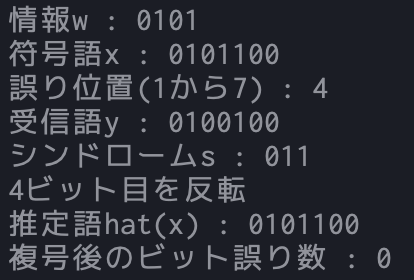
\includegraphics[scale=0.8]{kadai3_2_1.png}
    \end{center}
    \caption{プログラムの実行結果}
\end{figure}
\clearpage

\section{検討}
\subsection{課題1}
\begin{shadebox}
    なぜ(7,4)ハミング符号は1個誤りを訂正できるか。
\end{shadebox}
ハミング符号の生成多項式は$g(x)=x^3+x+1$であるから、
今回の冗長は3ビットなので、
情報系列$\boldsymbol{w}=(x_1,x_2,x_3,x_4)$としたとき、
冗長$\boldsymbol{c}=(c_1,c_2,c_3)$は次のようになる。
\begin{eqnarray}
    c_1&=&x_1 \oplus x_2 \oplus x_3 \nonumber\\
    c_2&=&x_2 \oplus x_3 \oplus x_4 \nonumber\\
    c_3&=&x_1 \oplus x_2 \oplus x_4 \nonumber
\end{eqnarray}
よって、情報系列$\boldsymbol{w}=(x_1,x_2,x_3,x_4)$に対して、
冗長$\boldsymbol{c}=(c_1,c_2,c_3)$は1対1対応に決まる。

したがって、
\begin{eqnarray*}
    H = \left[
        \begin{array}{rrrrrrr}
            1 & 1 & 1 & 0 & 1 & 0 & 0 \\
            0 & 1 & 1 & 1 & 0 & 1 & 0 \\
            1 & 1 & 0 & 1 & 0 & 0 & 1
        \end{array}
        \right]
\end{eqnarray*}
の転置を右から書けた値もただ一つに決まるので、
シンドローム$\boldsymbol{s}=(s_1,s_2,s_3)$は、ただ一つに決まる。

したがって、誤り箇所が分かるので1個の誤りを訂正できる。

\subsection{課題2}
\begin{shadebox}
    $2,3,...$個の誤りが発生するとどうなるか。
\end{shadebox}

$\boldsymbol{s}=\boldsymbol{y} H^T$において、
この計算式でシンドロームを計算するが、
$\boldsymbol{y}$が誤りを2つや3つ発生していても、
シンドローム$\boldsymbol{s}$は3ビットしか得られない。
つまり、$2^3=8$通りより、
誤りがないもしくは$1\sim 7$ビット目が誤っているとしか判定できない。
したがって、1個より大きい誤りが発生した場合は訂正はできない。

\clearpage
% 付録
\appendix
\section{付録}
\begin{lstlisting}[style = lstcpp,caption=kadai3\_3.cpp]
    //4619055 辰川力駆
    #include <random> // 乱数生成
    #include <stdio.h>
    #include <iostream>
    #include <iomanip>
    
    using namespace std;
    
    #define N 7         ///符号化後のビット数
    #define K 4         ///デジタル情報の分けるブロックのビット数
    #define seed 55     ///学籍番号下2桁
    #define SIM 1000000 ///シミュレーション回数
    
    mt19937 mt(seed); ///メルセンヌ・ツイスタ
    
    int main()
    {
        uniform_real_distribution<double> rand_real(0, 1);
        normal_distribution<double> rand_n(0, 0.3);
    
        int w[K];                  //4ビットの情報w
        int x[N];                  //7ビットの符号語x
        int e[N];                  //7ビットの雑音ベクトルe
        int y[N];                  //7ビットの受信語y
        int s[3];                  ///シンドロームs
        int bit_count = 0;         ///シミュレーションごとの毎回のビット誤り数を計算
        int total_bit_count = 0;   ///誤ったビットの総数
        int total_block_count = 0; ///ブロック単位の誤りの総数
        int EstimationPosition;    ///誤り位置推定場所
        double ep;                 ///誤り率
    
        cout << "# SIM:" << SIM << endl;
        cout << "#BSCの誤り率 #復号後ビット誤り率 #復号後ブロック誤り率" << endl;
    
        for (int k = 0; k < 5; k++)
        {
            ep = 0.005 + k * 0.004;
            total_bit_count = 0;
            total_block_count = 0;
    
            for (int sim = 0; sim < SIM; sim++)
            {
                bit_count = 0;
    
                for (int i = 0; i < K; i++) //K=4 ビットの情報 w を乱数を用いて生成
                {
                    w[i] = rand_real(mt) * 2;
                }
    
                for (int i = 0; i < K; i++) ///符号化により, w から x を生成
                {
                    x[i] = w[i];
                }
                x[N - K + 1] = w[0] ^ w[1] ^ w[2];
                x[N - K + 2] = w[1] ^ w[2] ^ w[3];
                x[N - K + 3] = w[0] ^ w[1] ^ w[3];
    
                for (int i = 0; i < N; i++) ///乱数を用いてN=7ビットの雑音ベクトルeを生成
                {
                    if (rand_real(mt) <= ep)
                    {
                        e[i] = 1;
                    }
                    else
                    {
                        e[i] = 0;
                    }
                }
    
                for (int i = 0; i < N; i++) //xとeの排他的論理和を計算してyとする
                {
                    y[i] = x[i] ^ e[i];
                }
    
                s[0] = y[0] ^ y[1] ^ y[2] ^ y[4]; //yから復号してxハット、wハットを得る
                s[1] = y[1] ^ y[2] ^ y[3] ^ y[5];
                s[2] = y[0] ^ y[1] ^ y[3] ^ y[6];
    
                int point = 0;
                for (int i = 0; i < 3; i++)
                {
                    point += s[i] * pow(2, 2 - i);
                }
                switch (point)
                {
                case 5:
                    EstimationPosition = 1;
                    break;
                case 7:
                    EstimationPosition = 2;
                    break;
                case 6:
                    EstimationPosition = 3;
                    break;
                case 3:
                    EstimationPosition = 4;
                    break;
                case 4:
                    EstimationPosition = 5;
                    break;
                case 2:
                    EstimationPosition = 6;
                    break;
                case 1:
                    EstimationPosition = 7;
                    break;
                default:
                    EstimationPosition = -1;
                    break;
                }
                if (EstimationPosition != -1)
                {
                    y[EstimationPosition - 1] = y[EstimationPosition - 1] ^ 1;
                }
    
                for (int i = 0; i < K; i++) //w と wハットを比較し、 ビット誤り数をカウント(つまり4ビットまでを見れば良い)
                {
                    bit_count += w[i] ^ y[i];
                }
    
                total_bit_count += bit_count;
    
                if (bit_count != 0)
                {
                    total_block_count += 1;
                }
            }
            cout << ep;
            cout << fixed << setprecision(8) << "        " << (double)total_bit_count / (K * SIM);
            cout << fixed << setprecision(6) << "          " << (double)total_block_count / SIM << endl;
            cout.unsetf(ios::fixed); ///体裁を整えている
        }
        return 0;
    }
    
\end{lstlisting}

%%%%%%%%%%%%%%%%%%%%%%%%%%%%%%%%%%%%%%%%%%%%%%%%%%%%%%%%%%%%%%
\end{document}